\documentclass[border=5mm]{standalone}
\usepackage{tikz}
\begin{document}
	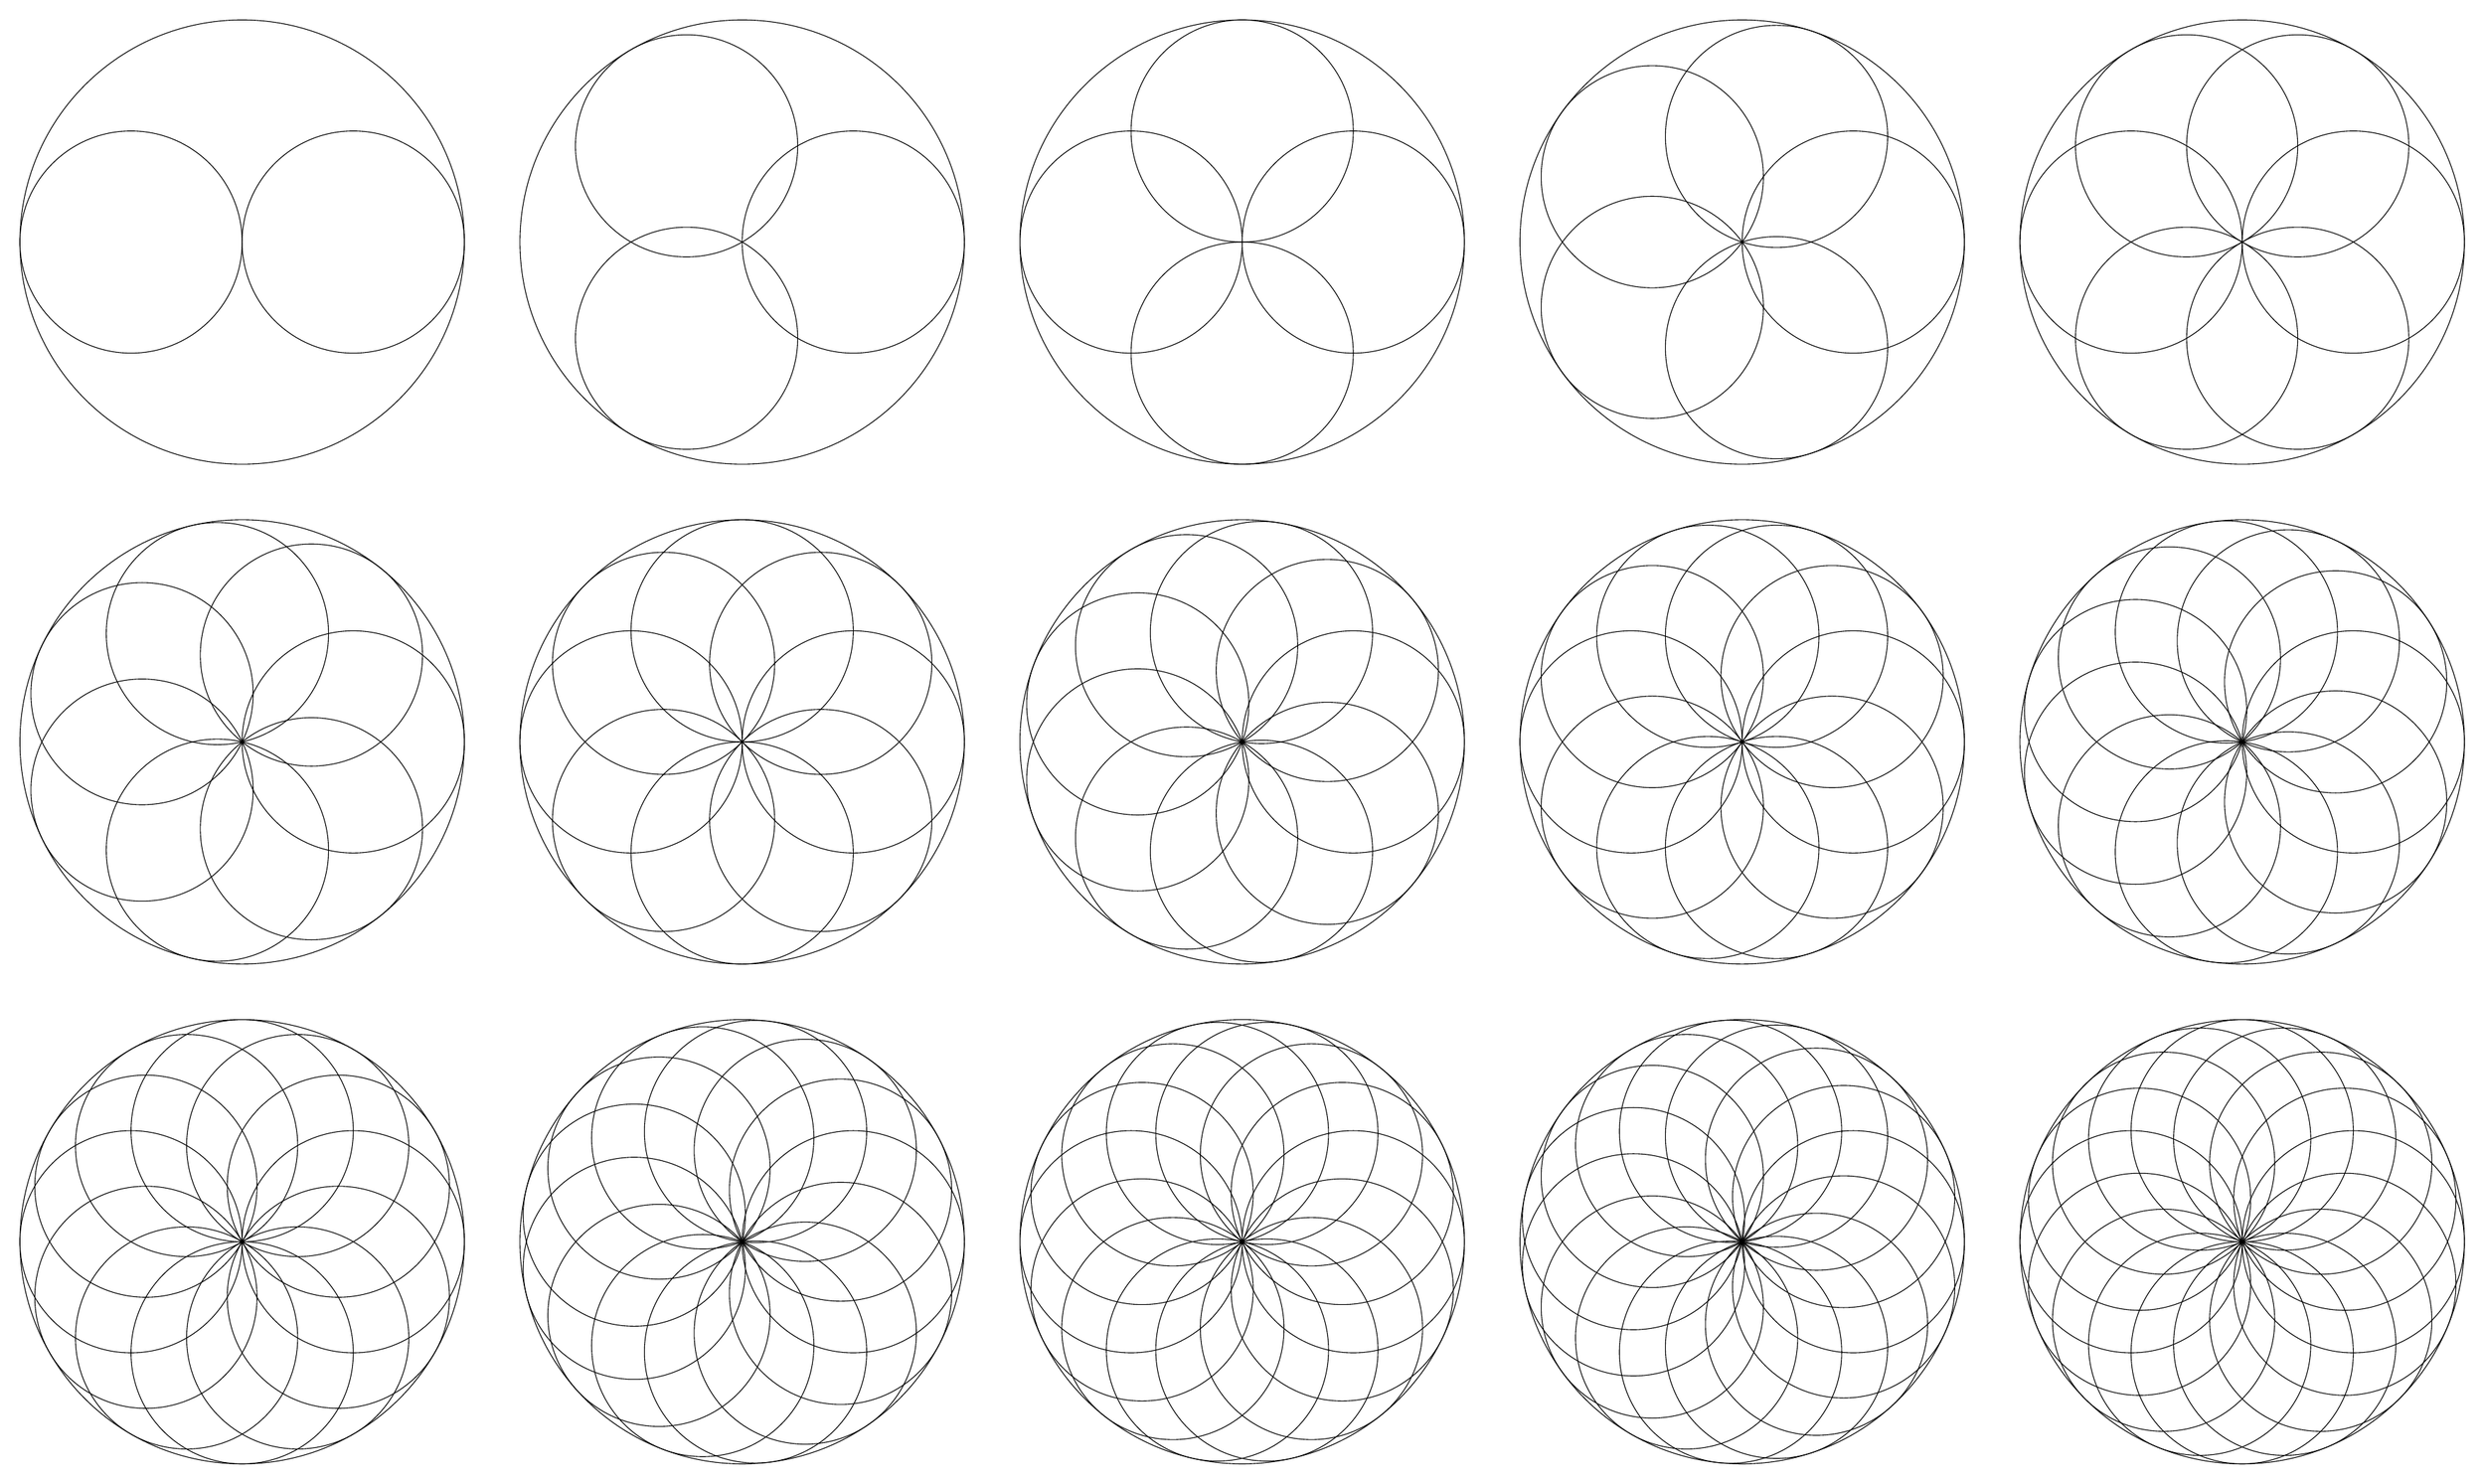
\begin{tikzpicture}[scale=1]
		\def\r{2}\def\col{5}
		\foreach \n in {2,...,16}{
			\pgfmathsetmacro{\xc}{mod(\n-2,\col)}
			\pgfmathsetmacro{\yc}{-div(\n-2,\col)}
			\foreach \i in {1,...,\n} 
			\draw (4.5*\r*\xc,4.5*\r*\yc)++({\i *360/\n}:\r) circle (\r);
			\draw (4.5*\r*\xc,4.5*\r*\yc) circle (2*\r);
		}
	\end{tikzpicture}
\end{document}